\documentclass{llncs}

\usepackage{graphicx}                                        % for pdf, jpeg, png and tif graphics
\usepackage{amsmath}                                         % for align
\usepackage{amssymb}                                         % for >= and <= signs
\usepackage{xfrac}                                           % for nice x/y fractions (sfrac)
\usepackage{tikz}
\usepackage{amsbsy}                     % for boldsymbol
\usepackage{upgreek}

\mathchardef\mhyp="2D    % define math mode hyphen

\allowdisplaybreaks[4]

\title{Deep feedback learning}

\author{Bernd Porr \and Paul Miller}

\institute{Glasgow Neuro, bernd,paul@glasgowneuro.tech}

\begin{document}

\maketitle

\begin{abstract}
\end{abstract}

\section{Introduction}

\begin{figure}[h!]
  \centering
  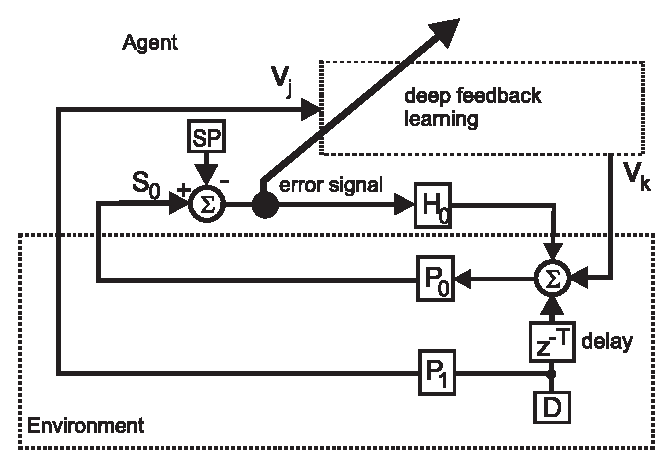
\includegraphics[width=0.75\columnwidth]{closed_loop}
  \caption{A closed loop system with a setpoint $SP$, transfer function $H$ and the
    environment $P_0$ which needs to work against unpredictable disturbances $D$.
    The error signal generated tunes a deep neuronal network which has inputs
    $v_j$ which predict the disturbances. The network tries to pre-empt these
    disturbances and generate an appropriate action $v_k$.
    \label{closed_loop}}
\end{figure}

\section{Closed loop learning}

Deep feedback learning operates in a closed loop scenario. Before we can describe
the actual deep feedback algorithm we need to put the algoritm into a closed loop
system. Fig.~\ref{closed_loop} shows the whole closed loop system with the deep
feedback learning as a black box for now. The main idea is that we have a fixed
closed loop which is able to fend off disturbances. For example this can be
an unexpected bend on a road or the sudden appearance of an enemy. The loop then
takes appropriate action to solve this disturbance, e.g. steering the car along
the road or shoots the enemy. In formal terms we have a setpoint $SP$ which
compares the input of organism to an input. If that input deviates from the
setpoint an action is generated with the transfer function $H_0$. This action
then eliminates the disturbance $D$ and arrives via the environmental
transfer function $P_0$ at the input again, thus, the loop is closed. However,
we are not so much interested in the particular design of the the closed loop
but that it generates an \textsl{error signal}. This error signal is non-zero
if a disturbance has happend. This error signal can now be used to tune our
deep feedback learning network.

The deep feedback learning network receives additional inputs which are able
to predict the disturbance and thus can prevent the trigger of the feedback
loop. These additional inputs are provided via the transfer function $P_1$
and represent the disturbance in a filtered form. For example a video camera
can provide images of the road ahead or that of the enemy. Deep feedback
learning has the task to take the error signal and tune its network
to generate an action which helps to minimise the error. In the next section
we are going to describe the deep feedback learning now how this can
compute the appropriate output. Note that deep feedback learning receives
its feedback via the environment so that it only learns if it has been
successful after its actions have travelled through the environment. Thus learning
evaluates if certain inputs to its network can be used to generate
appropriate actions and these are then slowly transformed into actions.
For that reason the error signal is propagated in a \textsl{forward} fashion
throught the network which will be presented next.

\begin{figure}[h!]
  \centering
  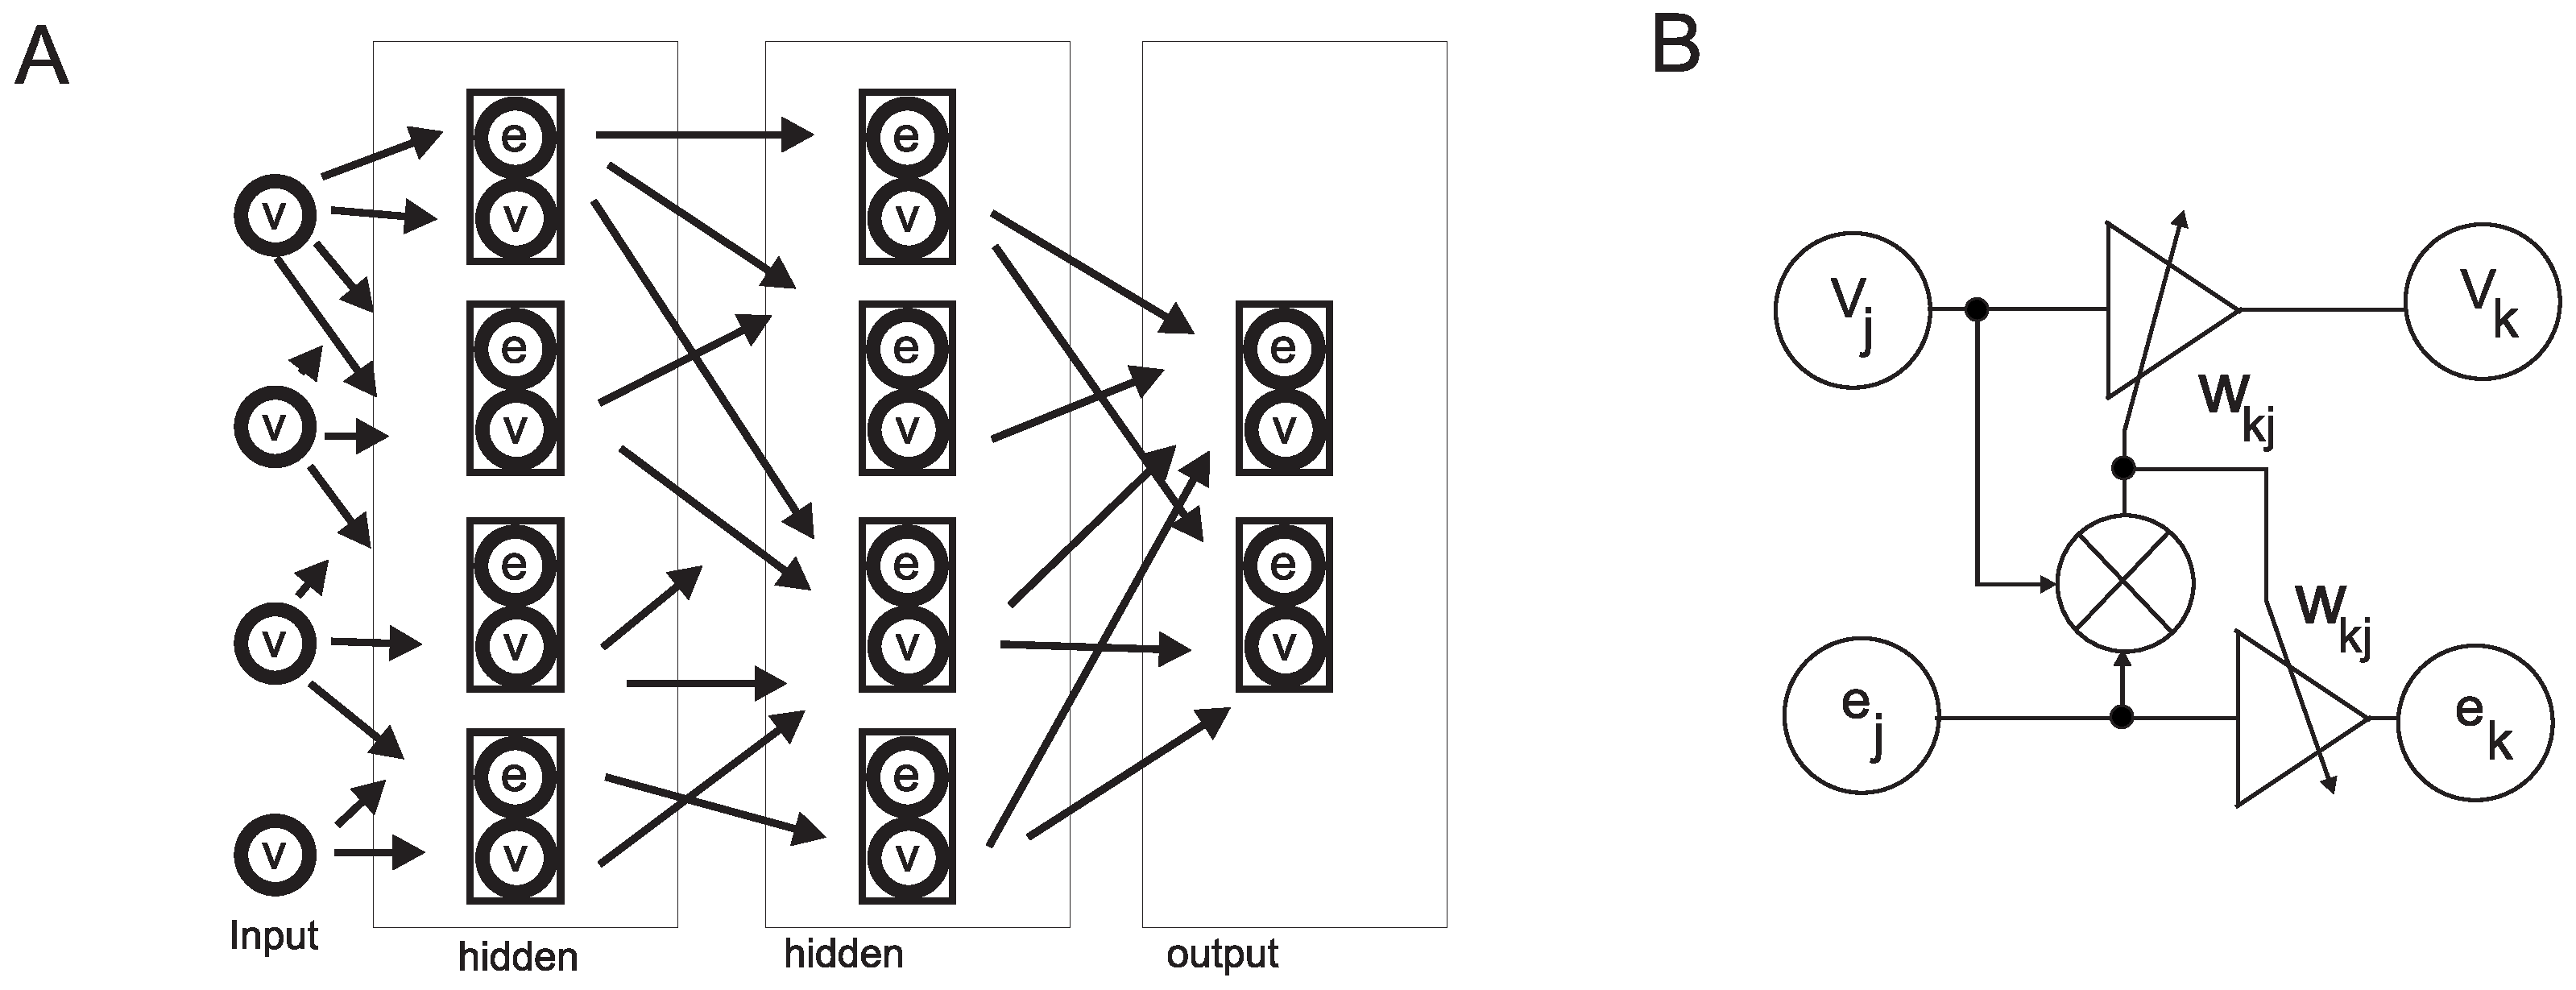
\includegraphics[width=\columnwidth]{netw_together}
  \caption{A) Overview of the network. Except for the input layer
    every neuron is a composite neuron with an activation $v$ and
    and an error term $e$. These are propagated through the network
    in a weighted fashion in parallel.
B) Computation in a single cell composite cell in the network.
    The presynaptic activities $v_k$ and error signals $e_k$ are used
    to perform correlation based learning and change the weight $w_{kj}$
    which weights both the activity and the error towards the next
    layer.\label{netw_together}}
\end{figure}


\section{Deep feedback learning}
We define a network with an input layer, hidden units and an output
layer which can all have different number of neurons (see
Fig~\ref{netw_together}A). However, in contrast to traditional
networks every layer (except for the input layer) consists of two
summation nodes: the actual activity and an error signal. These
are processed in two parallel streams.

Let us first focus on the calculation of the network activity and then
we deal with the error processing. We define a multi layered network
where every neuron is a standard computational unit which calculates
the weighted sums of its inputs and then sent through an activation
function:
\begin{equation}
  v_k = \Theta\left( \sum_i w_{jk} v_{j} \right) \label{act_sum}
\end{equation}
where the activity feeds from neurons in layer $v_j$ to neurons in layer $v_k$
and so forth. The activities are weighted by the weights $w_{jk}$
in a standard fashion.

The weight change is then calculated in a semi Hebbian fashion:
\begin{equation}
  w_{jk} = w_{jk} + \gamma v_j * e_k
\end{equation}
where $v_j$ is the presynaptic activity and $e_k$ is the error signal
attached to the postsynaptic neuron so that the correlation is
calculated between the input signals and the error signals. This is similar
to Hebbian learning but here the presynaptic term is the activity
and postsynaptic one is the error signal.

The error signal needs to be described in more detail how this
is propagated through the network. As described above the error
signal emerges from the feedback loop which is injected into the
network at its first hidden layer as the ``postsynaptic'' activity.
Since the 1st hidden layer directly receives its error signal this
can be computed instantly.

For the deeper layers the error signal is computed as a weighted
sum of the error signals from the previous layer:
\begin{equation}
  e_k = \frac{\left( \sum_j w_{jk} e_{j} \right) \Theta^\prime (v_k) }{\sqrt{\sum_j w_{jk}}}
\end{equation}
where the $\Theta^\prime (v_k)$ is the derivative of the activation
function $\Theta(v_k)$.

The computations performed in every layer are shown in
Fig~\ref{netw_together}B where we see that the activity $v_j$ is
weighted by the weight $w_{jk}$ and then summed up in the next
layer. The same happens for the error signal $v_j$ which is also
weighted by $w_{jk}$. Remember that for the 1st hidden layer this
error signal is just the injected error signal from the feedback loop
and is not the weighted sum.

Learning is then performed in three steps: first the activity is propagated through
the network, then the error signal is propagated via the same mechanism and then the
weights are adjusted. Thus, both the error
signal and the activity is propagated in a forward fashion through the network.
Learning itself is the ``Hebbian'' but by correlating the actual activation
and the error signal. 

\begin{figure}[h!]
  \centering
  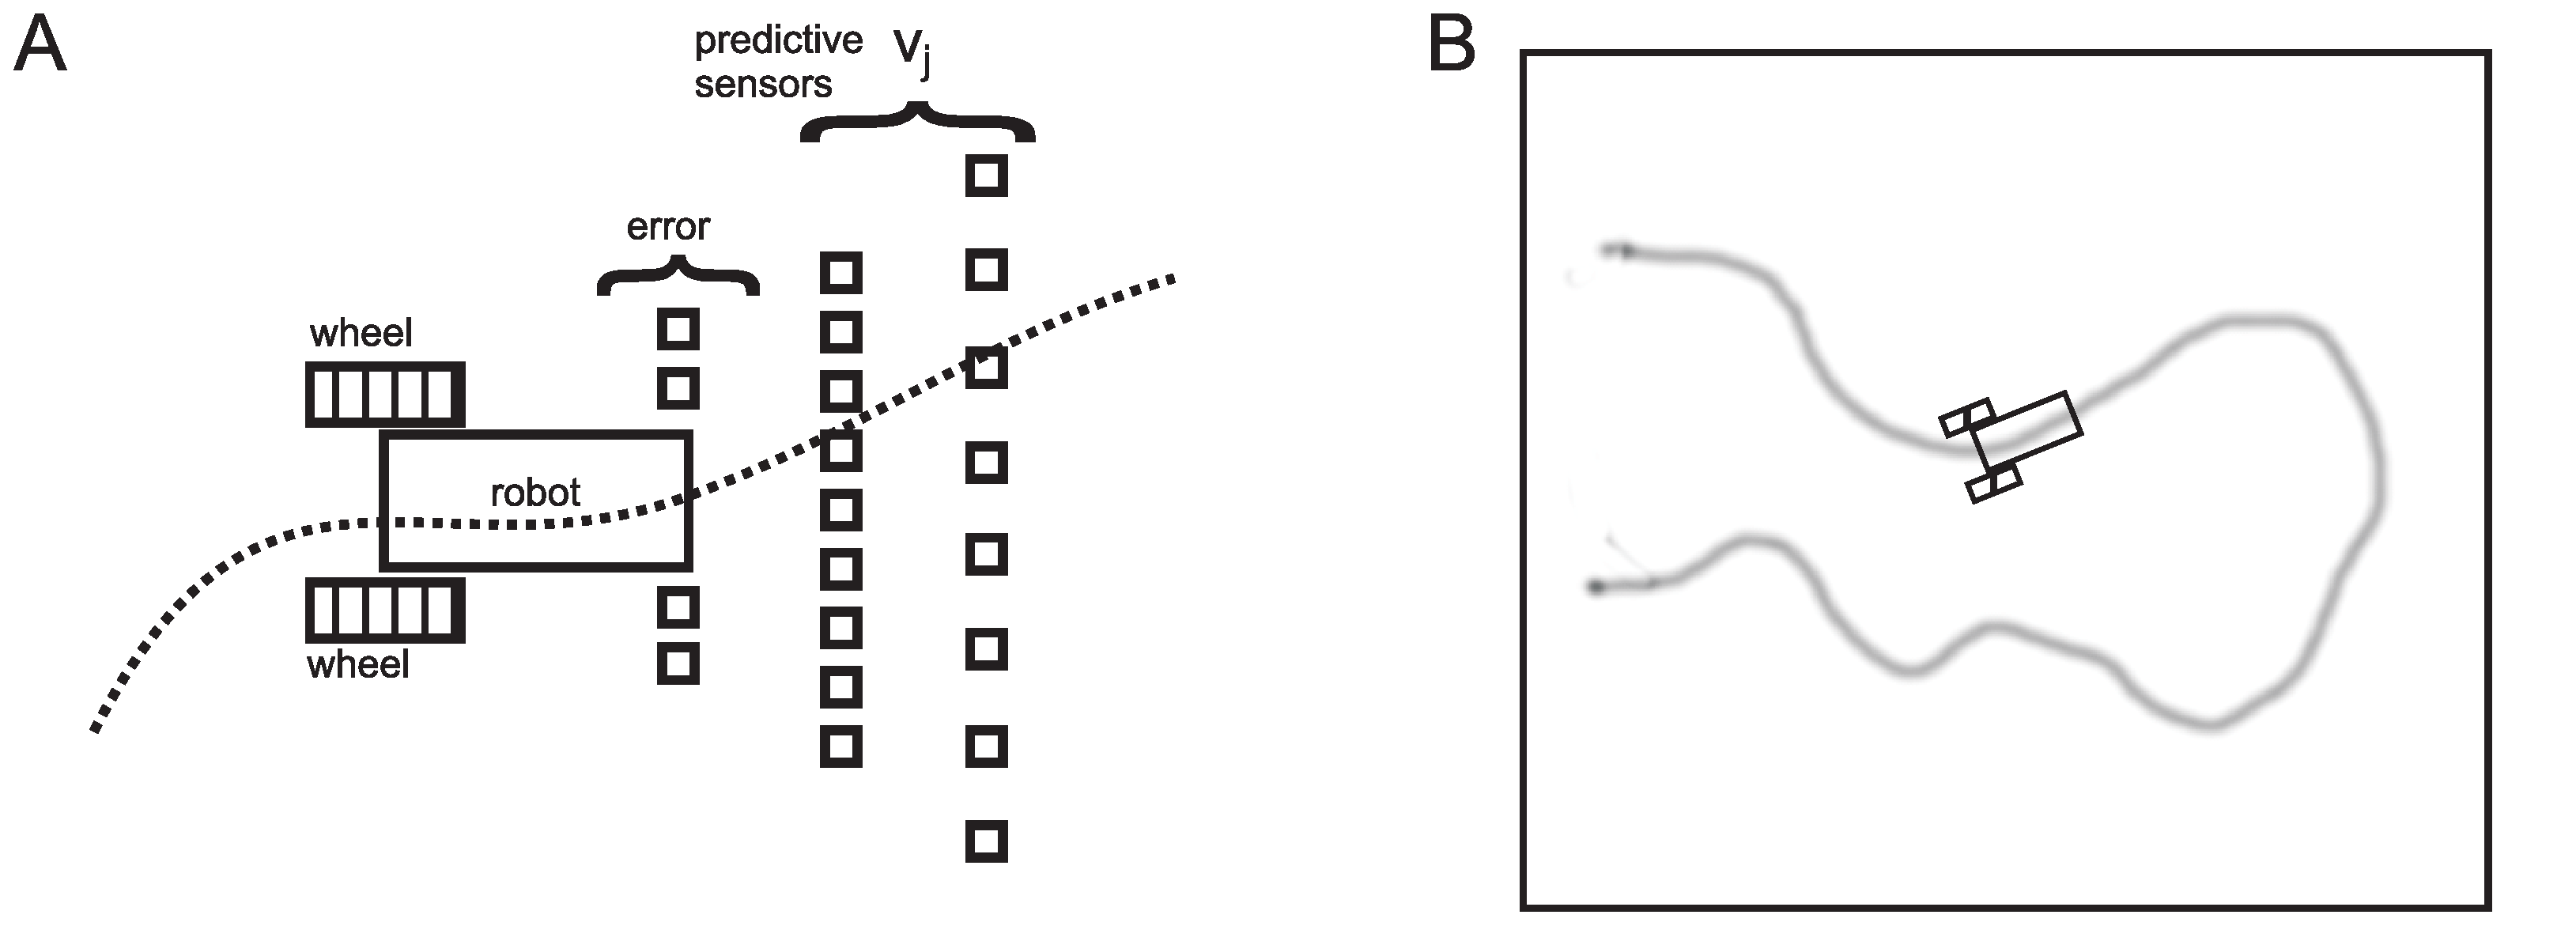
\includegraphics[width=\columnwidth]{linefollower_robot_playground}
  \caption{A) Robot setup. The robot is simulated with a updated
    version of enki for QT5 (https://github.com/berndporr/enki)
    where the line follower is using just the ground sensors of the
    robot to create the error signal and the predictive signals ($v_j$)
    for DFL. The robot has two wheels which speed is controlled
    by the feedback control and DFL.
    B) The line following scenario used for the simulations. The robot
    attempts to drive along the line and is reversed at the end of the
    line and the drives back. If it hits the boundaries of the playground
    it is also turned around.
    \label{linefollower_robot_playground}}
\end{figure}




\section{Line follower}
In order to demonstrate DFL we need a simple closed loop scenario which can be
improved with the help of our adaptive neuronal network. 
Fig.~\ref{linefollower_robot_playground} shows a simple line following robot which has the task to
follow the line as depicted in
Fig.~\ref{linefollower_robot_playground}B wheret the robot at the end the robot is reversed
and then drives it back in the other direction and so forth. The 4 ground sensors
in Fig.~\ref{linefollower_robot_playground}A right to both sides of the robot create
an error signal:
\begin{equation}
\mathrm{error} = (g_{l_1}+2 g_{l_2})-(g_{r_1}+2 g_{r_2}) \label{line_error}
\end{equation}
which then directly create a steering reaction to keep the robot on track by
controlling the speed of the wheels. Without taking into account the contribution
of our deep feedback learning output this yields: $\mathrm{leftSpeed} = s_0 + g error$ for the
left wheel and $\mathrm{rightSpeed} = s_0 - g error$ for the right wheel
where $s_0$ is the baseline speed of the robot and $g$ the feedback gain. We now
need to add the deep feedback learning circuit to it.

We now need to add our deep feedback learning circuit which uses the
predictive ground sensors where their outputs all feed into $v_j$ of
the input layer (see Eq.~\ref{act_sum}) after having been filtered bbb
fixme Filterbank bbb. We have two rows of sensors. One which is right
in front of the robot and another one which looks further ahead.

The output layer of our deep feedback learner with its activations
$v_k$ has 6 neurons ($k=0 \ldots 5$) which can be seen as soft
decision making units where 3 of them determine the change of the speed of
the wheel on the right and 3 of them the speed of the wheel on the
left which leads to the final formulas for the motor outputs:
\begin{eqnarray}
  \mathrm{leftSpeed} &=& s_0 + \underbrace{g\, \mathrm{error} + \left( 50 v_0 + 10 v_1 + 2 v_2 \right)}_{v_l} \\
                     &=& s_0 + v_l \\
  \mathrm{rightSpeed} &=& s_0 - \underbrace{g\, \mathrm{error} + \left( 50 v_3 + 10 v_4 + 2 v_5 \right)}_{v_r} \\
                     &=& s_0 - v_r
\end{eqnarray}
where $v_0, \ldots, v_5$ are the 6 outputs from the deep feedback learning network.
Note that neither the inputs nor the outputs are organised in a topographically
organised way. The network needs to find out with the help of the error signals
which sensor inputs $v_k$ will lead eventually to appropriate steering actions $v_j$.

In order to have a performance criterion which indicates a successful
run we have average the error Eq.~\ref{line_error}:
\begin{equation}
  \mathrm{error}_\mathrm{avg} =  \mathrm{error}_\mathrm{avg} + 0.001 (\mathrm{error} - \mathrm{error}_\mathrm{avg}) 
\end{equation}
and then squared it:
\begin{equation}
  \mathrm{error}_\mathrm{sq} =  \mathrm{error}_\mathrm{avg}^2 \label{line_sqerr}
\end{equation}
Remember that the learning tries to minimise the average error so that $\mathrm{error}_\mathrm{avg}$
should reach zero in an ideal scenario. Realistically it will fluctuate between negative and
postive vales because the driving will never be 100\% perfect. By squaring these fluctuations
we have a positive value which should decay and then stabilise at small values.


\begin{figure}[h!]
  \centering
  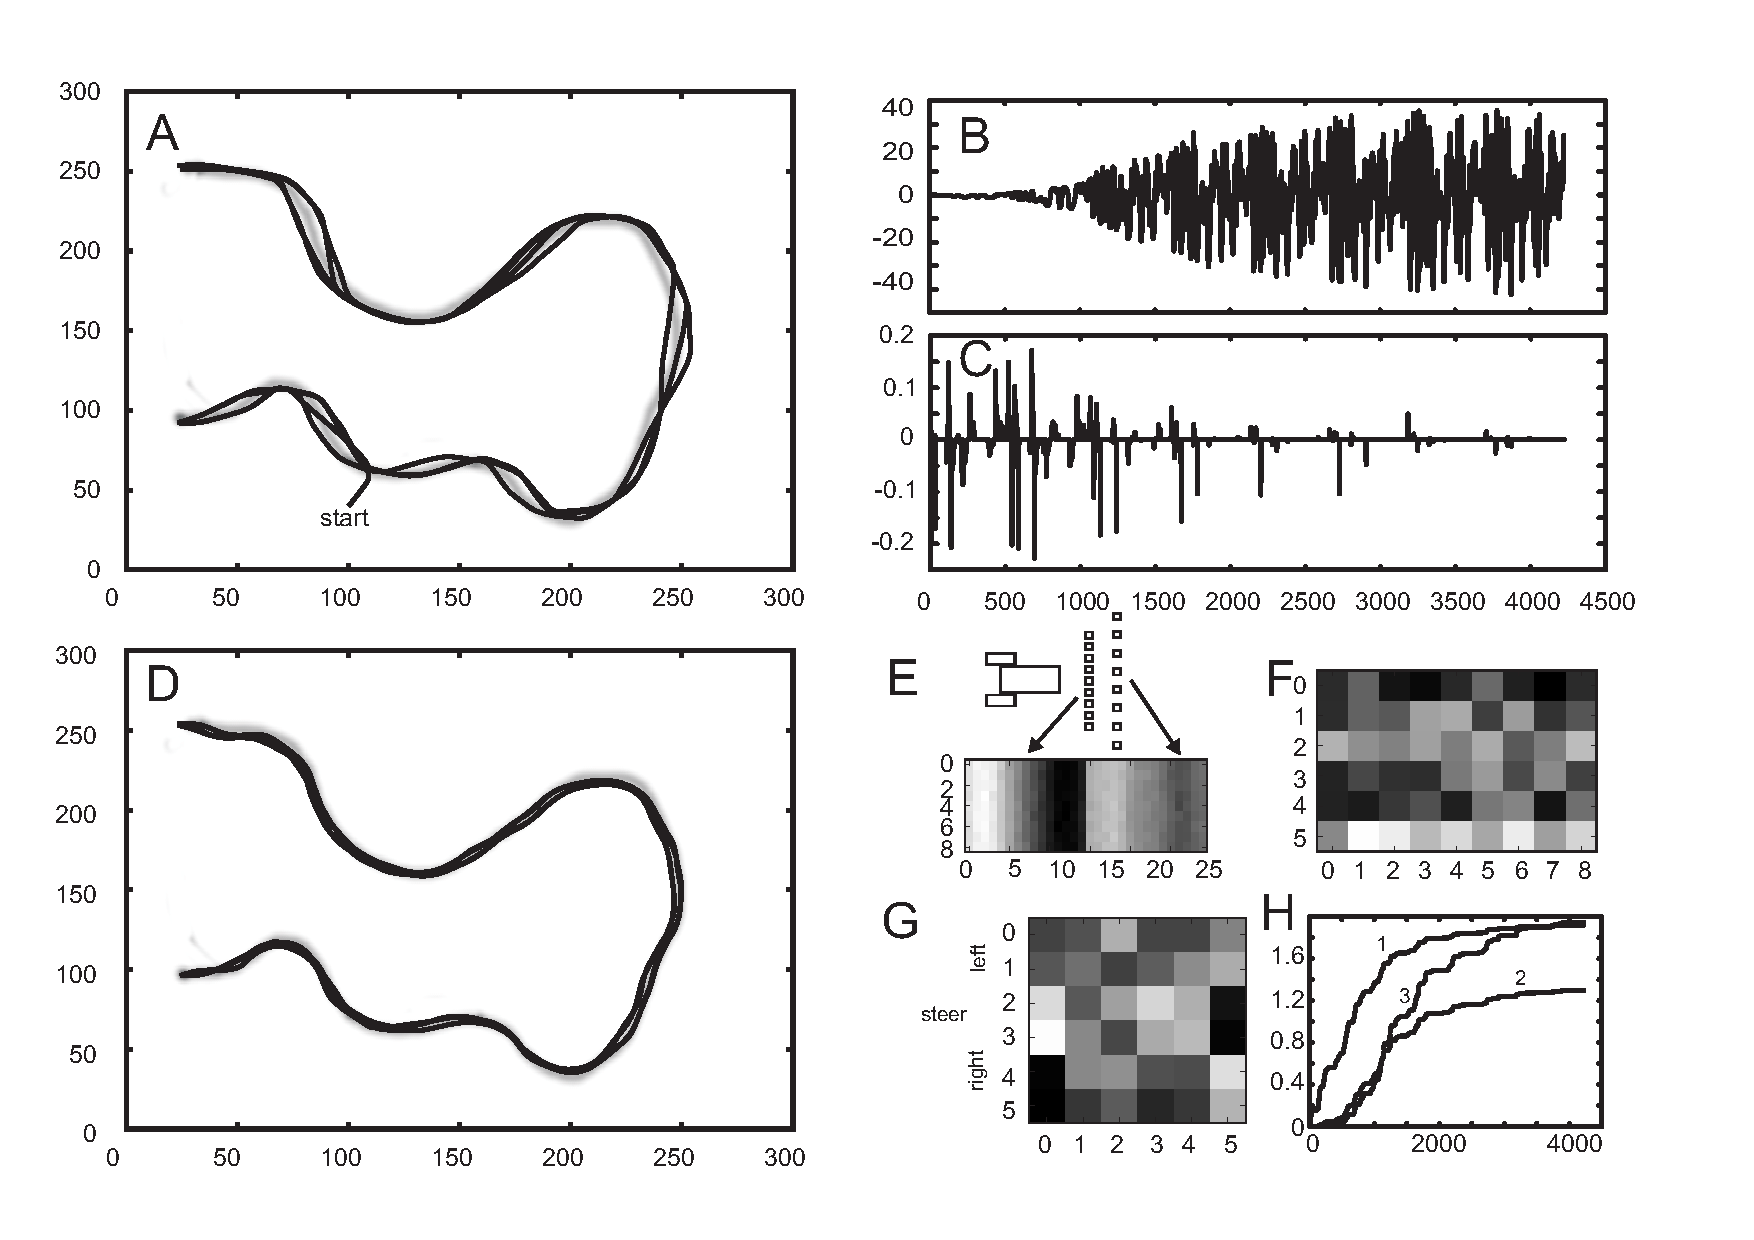
\includegraphics[width=\columnwidth]{line_results}
  \caption{Results of the linefollowing task. A) Shows the robot at
    the very start of the simulation run from time step 0 to 600.
    B) the difference between the robot wheel speeds just for the learned
    actions (i.e. the output of the dfl network): $v_l-v_r$.
    C) the error signal squared: $\mathrm{error}^2$.
    D) simulation run just before the end at 13400 to 14000 time steps.
    E-G show the weights of the different layers. The input neurons are on the x-axis
    and the output neurons are on the y-axis.
    E) the weights of the 1st layer, F) the weights of the 2nd layer and
    G) the weights of the output layer.
        H) shows the euclidean distance of the weights for each layer from their initial starting point.
    \label{line_results}}
\end{figure}



\subsection{Results}
Fig.~\ref{line_results} shows the results of a simulation run. In the panels
A) and D) we see the trajectory of the agent at the starts of the run and
at the end of the run afer 11400 time steps. While the agent in A) clearly
just follows the reflex reaction which leads to a large deviation from the track
in D) the agent follows closely the track and the deviation is minimal, thus
learning has been successful. The steering output of the DFL network are shown
in B) which generate the steering actions to keep the agent closely on track.
It can be seen that the network clearly slows down in the change of output.
C) is the squared error signal which shows that it quickly drops to near zero
and then only small components are left. E) is the weight matrix at the end
of learning of the 1st layer which correlates the error with the two rows of
predictive ground sensors $v_j$. F) is the weight matrix of the hidden layer and G)
the weigth matrix of the output layer. H) shows the eucledian distance of the
different layers from their starting position. Remember that learning is
always on and the learning rate is set to 0.0001 for the single run. See appendix
for the other parameters.

Let's first compare the trajectories at the start of learning. Figure
Fig.~\ref{line_results}A shows the robot right at the start. It locks
onto the track and then drives it back and forth with jerkey
movements. After $11,400$ time steps learning has turned the erratic
driving into a smooth driving scenario whree the robot only deviates
minimally from the track (Fig.~\ref{line_results}D). This smooth
steeting behaviour is generated by the DFL network which output is
shown in Fig.~\ref{line_results}B where the steering angle is shown.

The network learns to use the predictive signals from the sensors in
front of the robot to generate its steering which is shown in
Fig.~\ref{line_results}B.  The steering angle slowly becomes stronger and
then stabilises towards a final amplitude. Note that this is not
measured in degrees but this value is added and subtracted from the
speed of the robot wheels.

The squared average error in Fig.~\ref{line_results}C slowly decays
and then small remaining error spikes remain. This is mainly because
the robot is not able to learn one of the more steep bends (see
coordinate 120x50 in D) which always causes a spike in the error and
then the robot overcompensating which again causes learning in the
other direction and so on.

The weights of the different layers are shown in
Fig.~\ref{line_results}E-G.  The weights in the input layer
(Fig.~\ref{line_results}E) show a slow change from left to right as
expected. Remember that there are two rows of predictive ground
sensors in front of the robot which cause two different weight maps
which can clearly be seen. The inputs 0 to 14 correspond to the nearer
ground sensor and the inputs 15 to 31 correspond to the ground sensor
further ahead of the robot which can predict bends further
ahead. These feed then into the hidden layer Fig.~\ref{line_results}F
and from there into the output layer Fig.~\ref{line_results}G.

The weight development overall per layer over the time of learning
is shown in Fig.~\ref{line_results}H. It's interesting to note
that the input layer learns fastest and also its weights converge
quickest while the output layer learns at the slowest rate. Remember
that the error signal is weighted by the weights for the deeper
layers but normalised so that that learning happens at about the
same speed in every layer. However, the deeper layers show more
of a an exponential growths. The weights continue to grow at a slower
and slower pace but still continue because the robot is not completely
able to avoid its reflex and probably because the system is non-linear.
However, the error is very low even when the weights still change
substantially so that one could switch off learning if early stability
is required.



\begin{figure}[h!]
  \centering
  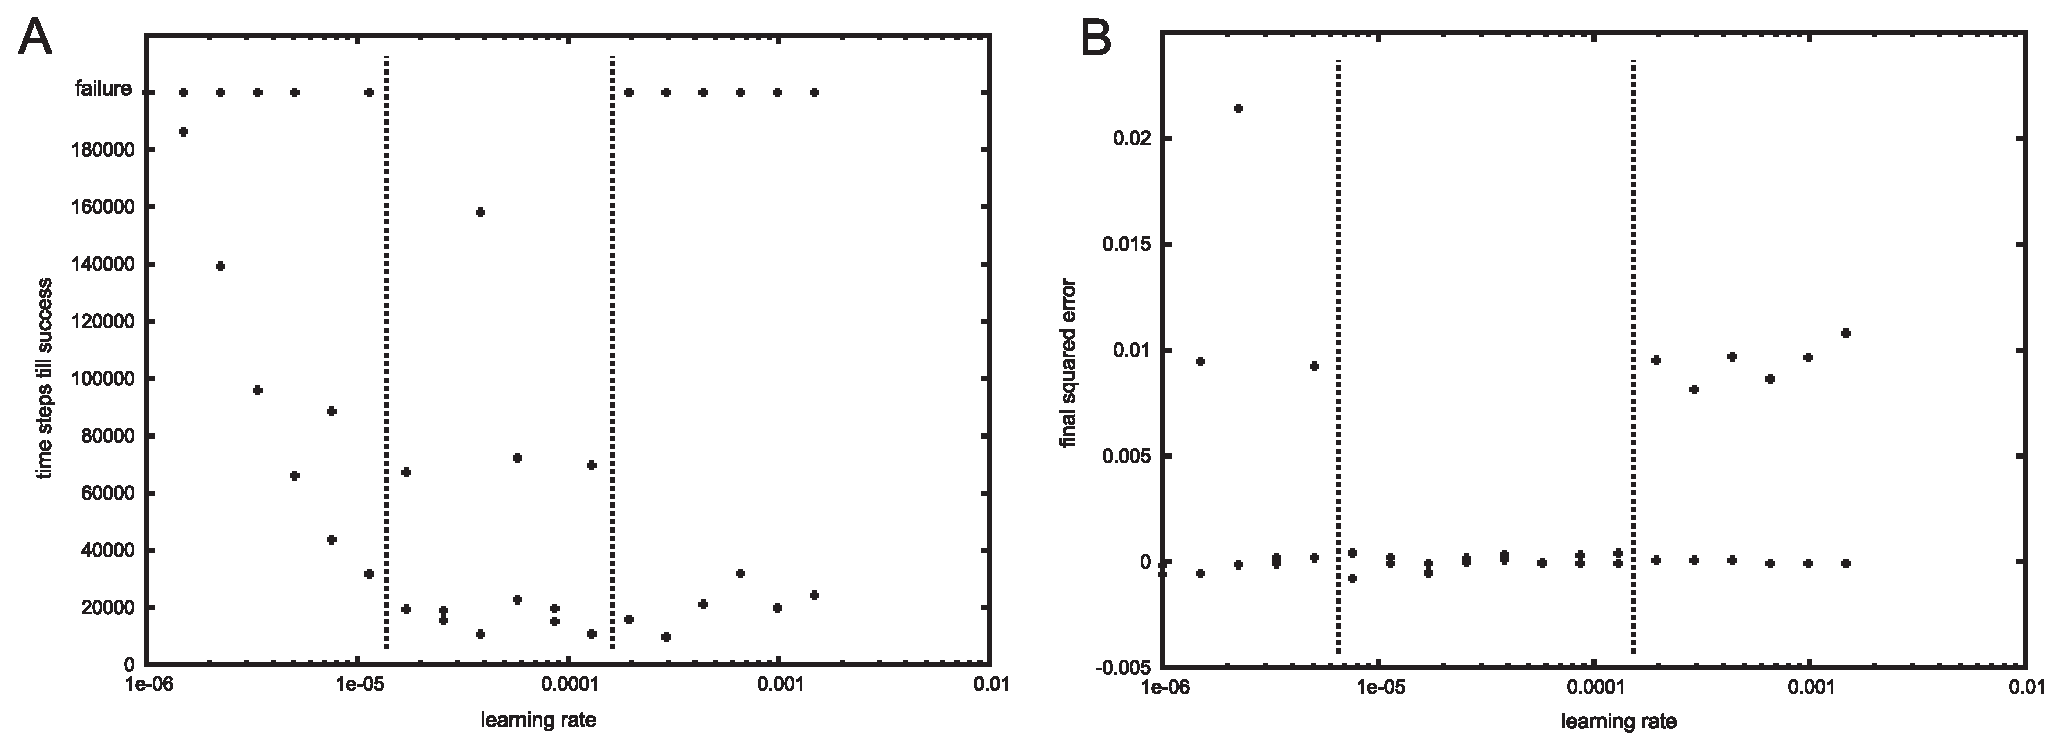
\includegraphics[width=\columnwidth]{line_stats}
  \caption{Statistics of the line following task. A) shows the relation between
    simulation steps against learning rate. For every learning rate two runs have
    been conducted with different random number seeds to test the dependence on the
    initialisation of the weights. The simulation was marked successful if the
    squared error Eq.~\ref{line_sqerr} stayed below $10^{-6}$ for more than $2500$
    timesteps. The simulation was aborted after $200,000$ time steps if this criterion
    hasn't been reached. Between the dotted lines every run has been successful.
    B) shows the final squared error for different learning rates and again between
    the dotted lines we have runs which resulted in low squared errors.
    \label{line_stats}}
\end{figure}

We have run statistics of the line follower where we varied the learning
rate over 4 orders of magnitudes and evaluated how long it takes to stay
below a certain error threshold (Fig.~\ref{line_stats}A) for a specified
time and the resulting squared error for these runs (Fig.~\ref{line_stats}B).
We see that the time to reach the criterion decreases with higher learning
rates and is stable between a learning rate of approx $10^{-5}$ and $10^{-4}$ and,
thus about one order of magnitude. In order to test if the network initialisation
plays a role for every learning rate the simulation was run with two different
random number seeds. It can be seen that in the stable region this results
in different times till success whereas outwidth the stable region about
half of the runs fail. For lower learning rates this might still become successful
in the end which suggests Fig.~\ref{line_stats}B where only three runs resulted
in non-convergence. At low learning rates the robot sometimes learns essentially
``open loop'' where the error signal has very little impact and thus learning
might drift very slowly into the wrong direction only to be corrected later on.
At very high learning rates the predictive learning turns into one shot
learning which also might learn accidentially the wrong behaviour. This is
then detrimental in numerous cases. In the optimal regime (between the dotted lines)
learning always reaches low error values. Overall it's interesting that lower
learning rates won't neccessary are better but that intermediate learning rates
perform best which does both, learning fast but slow enough so that the error
signal can correct mistakes.




\section{Shooter game}

In this scenario, we try to learn to play a first-person shooter purely from visual inputs. We use the Vizdoom (http://vizdoom.cs.put.edu.pl/) environment for this purpose, and train a controller to play against a single pretrained bot from Intel that ran in the Vizdoom 2016 competition. The setup was as follows:

Our bot’s only actions were to rotate in the plane, and shoot. We did also experiment with having our bot move around, but it is far more difficult to get effective learning trials. In the majority of cases, our bot would almost never see the enemy as it was facing towards the wall. We tried two different input representations - ‘flat’ input image vs assigning a spatial receptive field for each hidden unit. We found little difference in learning, so the flat form is reported here. We also experimented with a variety of temporal filters on the inputs, but found that the best results came from having no filters at all. We report the filterless version here. We created a custom Doom map that randomised spawn positions, so as to help generalise across visual inputs.

The images returned from Vizdoom are RGB. We rendered the enemy in blue, and formed a reflex signal by finding the bounding box of the pixels within a defined similarity of that colour. Note that the reflex is inherently noisy, as other events in the game are also rendered blue (e.g. the ‘flashes’ that happen when an ammo box respawns). The reflex also fails at times when the enemy is too distant or too close to the camera. For learning, we only supply the network with the greyscale image, so it is forced to discover purely spatial cues. The reflex is computed relative to the image centre, so a negative value implies the enemy is on the left. Shooting behaviour is entirely hardwired: if an enemy is detected within a threshold of the image centre, the bot fires. Instead of separate outputs for left and right, we have a single value produced by 3 neurons acting at different sensitivites:
\begin{equation}
\mathrm{rotation} = g_{err}\, \mathrm{error} + g_{net} \left( 10 v_0 + 3 v_1 + v_2 \right)
\end{equation}
where $v_0, \ldots, v_2$ are the network outputs.



\subsection{Results}

As before, we see that the controller outputs steadily increase over time. With a high value of $g_{net}$, the bot can make very rapid aiming movements. This has the advantage that the error can in principle be reduced very quickly; it also causes the bot to sometimes make large rotations even when the enemy is out of the field of view, which helps with exploration. On the other hand, it can cause the aiming to overshoot and oscillate around the target. 

Unlike the Line follower, in the shooting scenario it is not possible to drive the error to zero, as there are discontinuities when either bot respawns, and so the enemy will often abruptly appear somewhere in the image. A good measure of performance is simply how often our bot is killed vs how often it kills the enemy. In gaming, this is called the kill/death ratio, and we plot some smoothed KD curves in Fig.~\ref{shooter_results}



\subsection{Results}


\section{Discussion}

\bibliographystyle{splncs03}

\bibliography{sab_submission,isab,ours}

\end{document}



\begin{figure}[h!]
  \centering
  \includegraphics[width=\columnwidth]{arena_cct.pdf}
  \caption{A. Overview of the simulation environment. The arena has two markers, labelled R and B (red and blue), within   \label{fig:cct}
    }
\end{figure}

